\documentclass{beamer}

\usepackage[utf8]{inputenc}
\usetheme{Pittsburgh}
\usecolortheme{crane}
\usepackage{tikz}

\title{Hierarchical Topic Modeling}
\author{Ziv Epstein \\ \texttt{ziv.epstein@pomona.edu}}
\institute{Pomona College}
\date{\today}

\setbeamertemplate{navigation symbols}{}

\begin{document}
	
	\frame{\titlepage}
	
	\begin{frame}
		\frametitle{Topic Modeling}
		\begin{itemize}
			\item 	The world wide web has given us access to large quantities of text data, and often times there is too much text to read manually.
			\item The goal is to find automated techniques for understanding these large corpora.
		\end{itemize}
	
		\begin{definition}
			Given a corpus of documents $\mathcal{C} = \{d_1,d_2,\cdots,d_n\}$ with vocabulary set $\mathcal{V}$, a \alert{topic} $t_i$ is a frequency vector $\{f_1,f_2,\cdots, f_m\}$ where $|\mathcal{V}| = m$.
		\end{definition}
	\end{frame}
	\begin{frame}
		\frametitle{An example of Topic Modeling}
		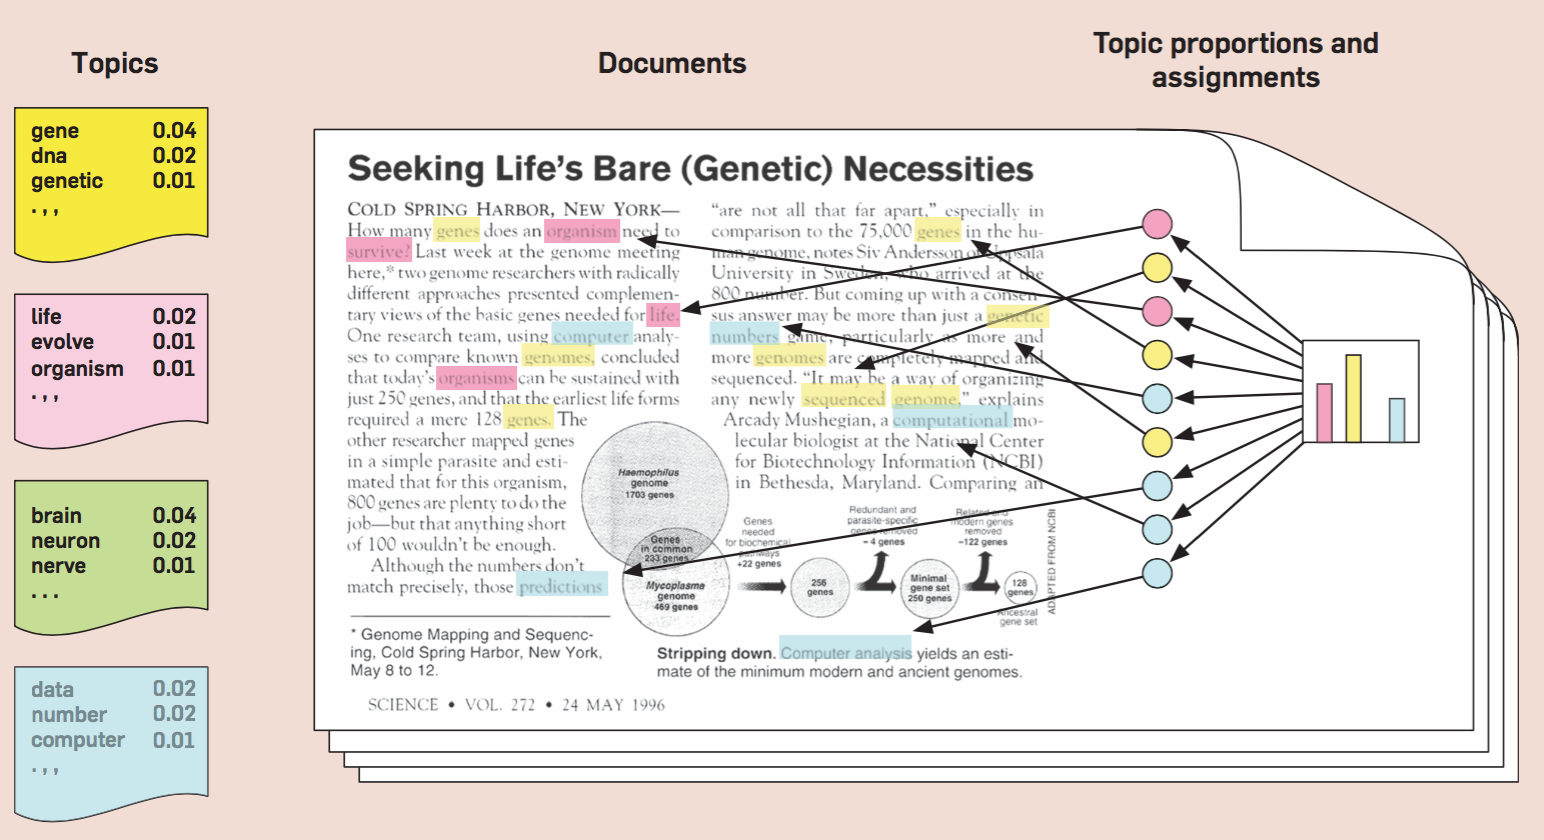
\includegraphics[width=10cm]{tmex}
	\end{frame}
		\begin{frame}
			\frametitle{Non-negative matrix factorization}
			Given $n$ documents with $|\mathcal{V}| = m$, let $X \in \mathbb{R}^{n \times m}$ be the word/document matrix.
				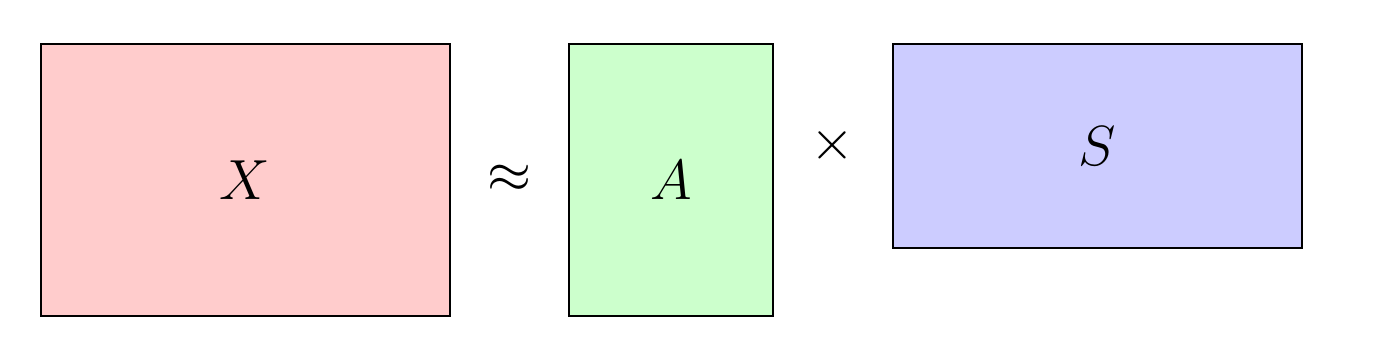
\includegraphics[width=10cm]{nnmf}
				
				Let $r$ be the inner dimension, the number of topics, such that $ A\in \mathbb{R}^{n \times r}$ is the document/topic matrix and $S\in \mathbb{R}^{r \times m}$ is the topic/word matrix.
				\begin{itemize}
					\item Nice linear algebraic intuition
					\item Fast implementations
				\end{itemize}
		\end{frame}
		\begin{frame}
				\frametitle{Hierarchical Topic Modeling}
				What if you want to impose some structure onto the topics, such as a hierarchy?
					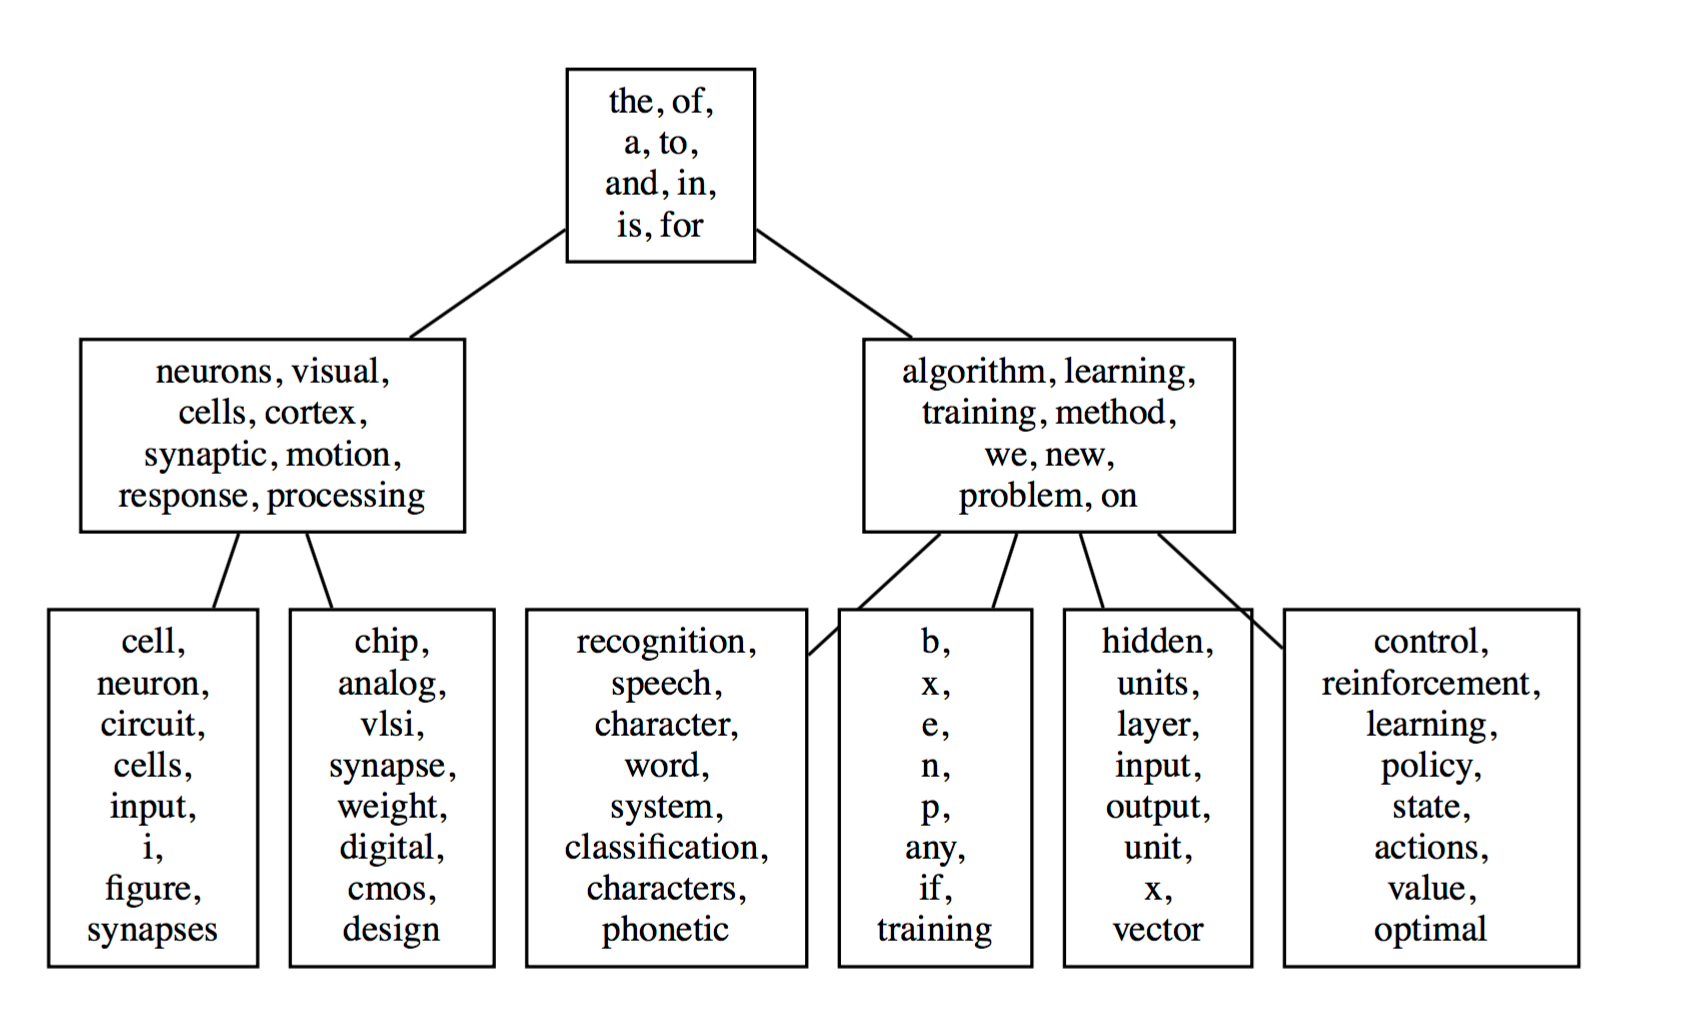
\includegraphics[width=10cm]{hierarchy}
				\end{frame}
				
					\begin{frame}
						\frametitle{An Algorithm for Building Hierarchical Topic Modeling}
						Insight: View the rows of $S$ (word embeddings of the topics) as points in $\mathbb{R}^m$. 
							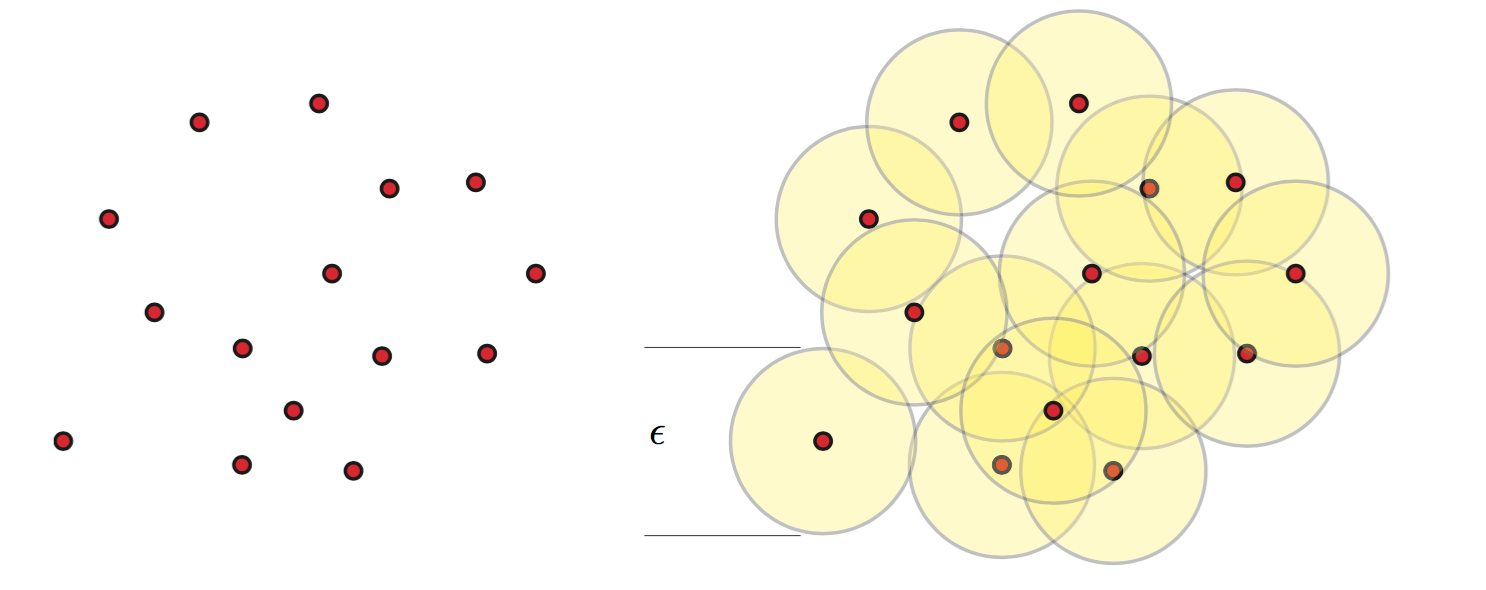
\includegraphics[width=10cm]{growth}
							
							Grow $\epsilon$-balls around each point, and merge leaves when $\epsilon$-balls overlap.
					\end{frame}
					\begin{frame}
						\frametitle{Interactive Demo}
						\url{http://www1.cmc.edu/pages/faculty/BHunter/ziv.html}
					\end{frame}
					
						\begin{frame}
							\frametitle{Deep Semi Supervised NNMF}
							Quick Review of Neural Networks
	\begin{figure}
		\centering
			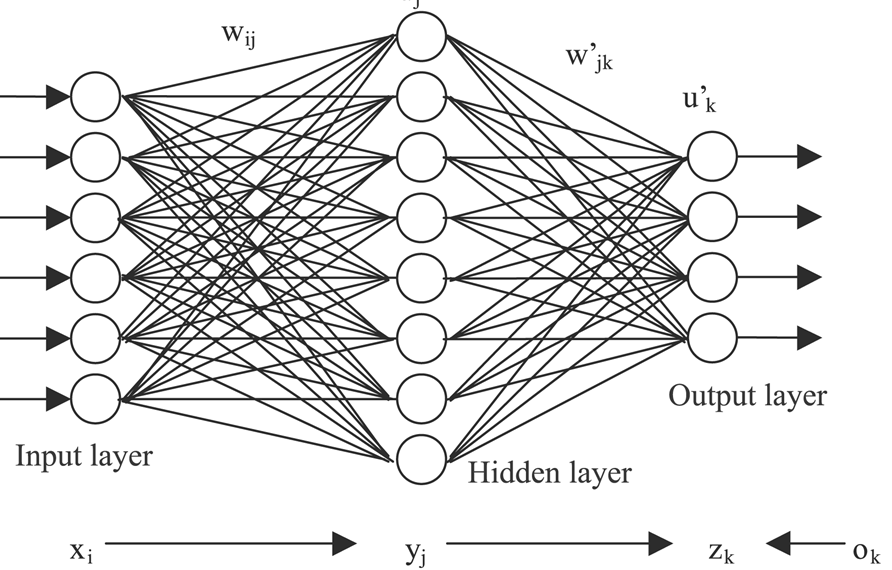
\includegraphics[width=9cm]{NeuralNetwork}
	\end{figure}

	
	Can be thought of as a matrix equation
	\begin{equation*}
	\overrightarrow{output} = \sigma_2 (W'(\sigma_1(W(\overrightarrow{input})))) 
	\end{equation*}
						\end{frame}
							\begin{frame}
								\frametitle{Deep Semi Supervised NNMF}
								Instead of only factoring $X \approx S \times A$, we instead recursively factor $A_i$ into $S_{i+1}$ and $A_{i+1}$.
								
								For example, 
								
\begin{align*}
X = S_1A_1\\X = S_1S_2A_2\\ \vdots \\X = S_1S_2 \cdots S_n A_n
\end{align*}
Key insight : We could already do this, but neural network optimization scheme gives us a robust way to learn $S_i$ 
									\end{frame}
									\begin{frame}
								Example: Let $X$ be a matrix of faces. Decompose $X$ into $Z_1 \times Z_2 \times Z_3 \times H_3$. Learns hierarchy of features.
								\begin{figure}
									\centering
										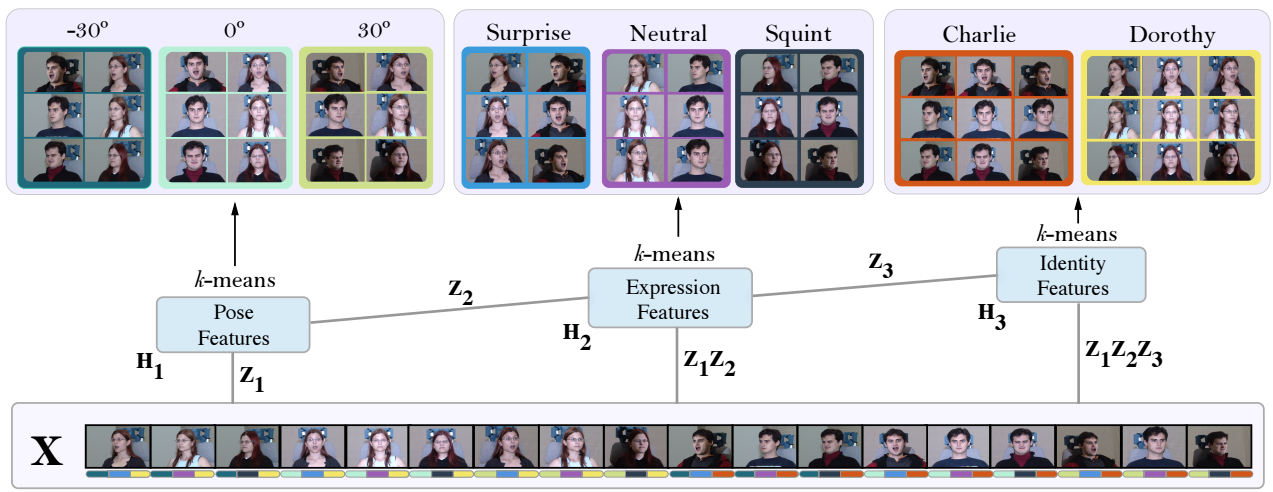
\includegraphics[width=10cm]{dsnnmf}
								\end{figure}
									Now let's apply it to topic modeling!
							\end{frame}
\end{document}